\documentclass[tikz,border=2pt]{standalone}
\usepackage{amsmath}
\usepackage{tikz}

\begin{document}
% A ∪ B: everything that belongs to A, to B, or to both (whole shaded region).
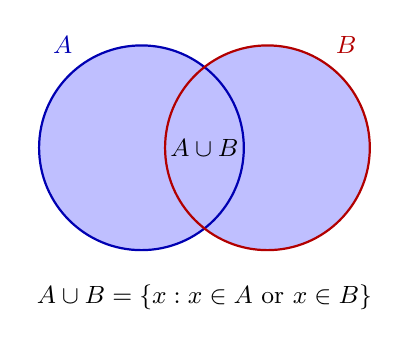
\begin{tikzpicture}[every node/.style={font=\small}]
	\fill[blue!25] (0,0) circle (1.3);
	\fill[blue!25] (1.6,0) circle (1.3);
	\draw[thick, blue!70!black] (0,0) circle (1.3);
	\draw[thick, red!70!black] (1.6,0) circle (1.3);
	\node[blue!70!black] at (-1.0,1.3) {$A$};
	\node[red!70!black] at (2.6,1.3) {$B$};
	\node at (0.8,0) {$A\cup B$};
	\node at (0.8,-1.9) {$A\cup B=\{x : x\in A \text{ or } x\in B\}$};
\end{tikzpicture}
\end{document}
